\chapter{A Geometric Perspective of Economic Engineering}
\label{chap:symplectic_economics}

The discipline of economic engineering is a very new one. The theoretical foundations have been developed over the past few years at the Delft Center of Systems and Control, primarily by prof. em. Mendel,  in combination with the contributions of several theses that have been recently written about the subject \cite{Hutters2020,Kruimer2021,VanArdenne2020,Manders2019}. Economic engineering aims to use tools from various engineering disciplines and physics to improve the predictive power of (macro)economic models.

In economic engineering, \emph{domain-neutral} modeling techniques such as bond graph modeling are used to construct models for economic systems. This is done based on analogies between economics and mechanical and/or electrical engineering. This results in dynamic gray-box models that rely on past data only for the identification of their parameters but not for the dynamics of the model itself. These gray box models are what sets economic engineering apart from other disciplines that produce economic models, such as econometrics.

In this chapter, we focus on the theoretical foundations of economic engineering, particularly its relation to symplectic manifolds and Hamiltonian and Lagrangian mechanics. The theoretical contributions in \Cref{chap:geometric_structures} are formulated exclusively in terms of concepts from classical mechanics, but the analogies provided in this chapter allow to extend the results in \cref{chap:geometric_structures} to the economic domain as well.

The structure of this chapter is as follows. First, in \cref{sec:symplectic_ee}, we explain the relevance of symplectic manifolds in economic engineering. Second, we first provide economic engineering analogies for Lagrangian mechanics in \cref{sec:lagrangian_ee}. Although \cref{chap:geometric_structures} is written from the Hamiltonian perspective, the Lagrangian formalism provides a more intuitive introduction to the economic engineering analogies. Finally, in \cref{sec:hamiltonian_ee} we explain the role of Hamiltonian mechanics in economic engineering and motivate why dissipative elements are an essential part of economic systems that must properly be dealt with.

\section{Symplectic manifolds in economic engineering}
\label{sec:symplectic_ee}
A collection of goods forms the basis of any economic system. These goods can be physical (e.g., bushels of wheat) but also more abstract notions such as capital in the financial analogy \cite{Kruimer2021}. The \emph{economic configuration space} \(Q\) is analogous to the configuration space of mechanics and consists of all the possible combinations of goods in the economy. 
Hence, in economic engineering, the goods are analogous to the \emph{(generalized) positions} in classical mechanics. 

The natural coordinates for this space are the number of each of the goods in the economic system, denoted by \(q = (q^1, q^2, \ldots, q^n)\), also called \emph{stock levels}. We say that each of these coordinates is measured in units of \emph{quantity}, denoted by `\(\qty[\si{\quantity}]\)'. 

In many cases, the economic configuration manifold is simply a vector space containing all the goods, subject to a total constraint on the total \emph{endowment} for each of the goods (i.e., the total number of goods available). This is also referred to as an \emph{Edgeworth box} in the two-dimensional case. However, we will not assume in general that $Q$ is a vector space, for it may be constructed from holonomic constraints imposed on a larger space.

The tangent space \(\tspace{x}{Q}\) to a point \(x\) in \(Q\) is the vector space of differential changes in goods, also called the \emph{flow of goods}. A vector in the tangent space is denoted by \(\vec{\dot{q}} = (\dot{q}^1, \dot{q}^2, \ldots, \dot{q}^n)\). It is important to distinguish between a flow of goods and an absolute amount of goods. From a mathematical perspective, the former is a vector in the tangent space, and the latter is a point in the economic configuration manifold. This distinction is often not given much attention in economics but is fundamental in economic engineering.

The \emph{dual space} of \(\tspace{x}{Q}\) is the cotangent space \(\ctspace{x}{Q}\) containing all the linear functions that map vectors in the tangent space to a real number. This is the natural setting of the \emph{prices} in the economy: as a function, they assign a \emph{value to a change in goods}. These prices are measured in units of currency per quantity, i.e. \(\qty[\si{\money \per \quantity}]\). A covector in the cotangent space is denoted by \(\vec{p} = (p_1, p_2, \ldots, p_n)\). The action of a price covector on a vector measuring the change in goods is (observing the summation convention):
\begin{equation}
    \vec{p}(\vec{\dot{q}}) = p_i\,\dot{q}^i,
\end{equation}
i.e., it produces the total value associated with this change in goods.

The \emph{cotangent bundle} \(\ctbundle{Q}\) of the economic configuration manifold is the space of prices and quantities: we call it the \emph{economic phase space}. Like in mechanics, a point in this space determines the state of the economic system: points in this space specify the amount of each of the goods in the system and their associated price.

The economic phase space has a natural structure that pairs each price coordinate to the associated stock level coordinate. From a mathematical perspective, this is equivalent to the fact that the cotangent bundle of any manifold has a 1-form canonically defined on it: the Liouville form (also called tautological 1-form or canonical 1-form), defined as
\begin{equation} 
    \theta \coloneq  p_i \dd{q}^i.
\end{equation}
Even more so than in mechanics, this Liouville 1-form has a very intuitive interpretation in economic engineering: it relates the goods and their prices. When integrated over a curve in \(\ctbundle{Q}\), it measures the total accumulation of value along that curve.

The (negative of) the exterior derivative of the Liouville form is a \emph{symplectic 2-form} \(\omega\):
\begin{equation}
    \omega \coloneq -\dd{\theta} = \wedgep{\dd{q}^i}{\dd{p}_i}.
\end{equation}
When integrated over, this form measures the \emph{oriented area} in the economic phase space, with units of currency \([\si{\money}]\). This quantity is analogous to \emph{action} in classical mechanics. The symplectic 2-form relates every price to the associated stock level and thereby encodes the fundamental structure of the economic phase space.  

The link between symplectic geometry and economics has been recognized by (more mathematically inclined) researchers outside the field of economic engineering as well, most notably \citet{Russell2011} and \citet{Swierstra2014}.

The role of symplectic geometry in economics begs the question of whether the concepts of Hamiltonian mechanics can also be applied to economic dynamical systems. In the field of economic engineering, we argue that this is indeed the case. To explain how this works, we start from Lagrangian mechanics, after which we transition to Hamiltonian mechanics.

\section{Lagrangian mechanics in economic engineering}
\label{sec:lagrangian_ee}

The \emph{Lagrangian} is a function on the tangent bundle of the configuration manifold:
\begin{equation}
     L : \tbundle{Q} \to \real.
\end{equation}
Lagrangian mechanics is based on \emph{Hamilton's principle} which states that the physical motion \(\gamma: \interval{t_0}{t_1} \to \tbundle{M}\) is the one for which the \emph{action functional} $\mathscr{A}$.
%\begin{eqbox}{Action functional}
%    The action functional of a curve $\gamma$ is defined as:
\begin{equation}
    \mathscr{A}[\gamma] \coloneq \int_{t_0}^{t_1} (L\circ\gamma)\dd{t}
\end{equation}
%\end{eqbox}
is stationary\footnote{Although often referred to as the `Principle of \emph{minimum} action', this is inaccurate: Hamilton's principle only asserts that the first variation of the functional vanishes, which does not necessarily imply a minimum.} \cite{Arnold1989}.

A necessary and sufficient condition for a curve to satisfy Hamilton's principle is given by the set of \(n\) \emph{Euler-Lagrange equations}:
\begin{equation}
    \dv{}{t}\qty(\pdv{L}{\dot{q}^i}) - \pdv{L}{q^i} = 0.
\end{equation}

In economic engineering, Hamilton's principle is interpreted as an economic agent minimizing hir or her \emph{disutility}, in practice often considered to be the \emph{cost}. The interpretation of the Lagrangian function is then the \emph{running cost} or \emph{running disutility}. This Lagrangian therefore has units of currency per time, e.g. \(\qty[\si{\money \per \year}]\).

As mentioned, the Lagrangian is a function of the flow of goods \(\dot{\vec{q}}\) and the stock levels \(q\). The partial derivative of the Lagrangian with respect to the flow of goods is equal to the \emph{price vector}:
\begin{equation}
    p_i \coloneq \pdv{L}{\dot{q}^i}. 
\end{equation}
This means that prices and flows of goods are \emph{conjugate variables}. Intuitively, the prices are the marginal increase in cost with respect to a marginal change in the flow (say, demand) of goods.

\subsection{Kinetic energy} When the Lagrangian depends quadratically on the flow of goods (analogous to kinetic energy), the price and the flow of goods are linearly related by an \emph{elasticity}: this is the typical picture of a supply and demand curve. We have:
\begin{equation}
     p_i = m_{ij} \dot{q}^j,
\end{equation}
where the \(m_{ij}\) are referred to as \emph{price elasticities}. In the simplest of cases, the \(m_{ij}\) form a diagonal matrix, and every good has its price. However, any cross-terms appearing in the elasticity matrix represent the marginal elasticity of one good relative to another. These cross terms encode the effect of \emph{substitution} of one good for another. The matrix of price elasticities is analogous to the (inverse) mass matrix in classical mechanics.

In mechanics, the part of the Lagrangian that depends on \(\dot{\vec{q}}\) is called the \emph{kinetic co-energy}\footnote{We make the distinction between the kinetic energy \(T\) and co-energy \(T^*\): they are dual representations related through the Legendre transform. Because work is the integral of force over distance, kinetic energy is naturally represented in terms of \emph{momentum}, rather than velocity, for which we need to apply the Legendre transform first \cite{Jeltsema2009}. The difference between the kinetic energy and kinetic co-energy is illustrated by \cref{fig:kinetic_energy}.} \(T^*\):
\begin{equation}
    T^* = \frac{1}{2}m_{ij}\dot{q}^i \dot{q}^j.
\end{equation} 
The kinetic co-energy is equivalent to the \emph{cost} associated with a flow of goods: the factor of one-half is there to subtract the market surplus from the total expenditure (which is equal to \(\vec{p}(\dot{\vec{q}})\)).

\begin{figure}
    \centering
    \begin{tikzpicture}

    \draw[thick,->] (-1,0) -- (5,0) node[anchor=west] {$\dot{q}\:\qty[\si{\quantity \per \year}]$};
    \draw[thick,->] (0,-1) -- (0,5) node[anchor=south] {$p\:\qty[\si{\money \per \quantity}]$};
    \draw[ultra thick,accent1, name path = S] (0,0) -- (5,5) node[anchor=west]{};

    \draw[thick, dashed, name path = dv] (4.5,0) -- (4.5,4.5); 
    \draw[thick, dashed, name path = dp] (0,4.5) -- (4.5,4.5); 
    \tikzfillbetween[of = S and dp]{accent1, opacity=0.4};
    \tikzfillbetween[of = S and dv]{accent1, opacity=0.2};

    \draw[dashed] (0,3) node[anchor=east]{$\dd{p}$} -- (3,3); 
    \draw[dashed] (0,3.3) -- (3.3,3.3) ;

    \draw[dashed] (3,0) node[anchor=north]{$\dd{\dot{q}}$} -- (3,3); 
    \draw[dashed] (3.3,0) -- (3.3,3.3) ; 

    \node at (2,0.5) (Tv) {$T^*(\dot{q})$};
    \node at (1,2) (Tp) {$T(p)$};


\end{tikzpicture}

    \caption{The difference between kinetic energy and co-energy. Kinetic energy is a function of momentum, and kinetic co-energy is a function of velocity. The two are numerically equivalent for this particular relation between momentum and velocity. Figure courtesy of B. \citet{Krabbenborg2021}.}
    \label{fig:kinetic_energy}
\end{figure}

Traditionally, microeconomics makes the distinction between \emph{firm theory} and \emph{consumer theory}. In economic engineering, we dispense with this explicit distinction, for we argue that they are fundamentally based on the same mathematical principles. However, it is important to keep in mind that the situation for firms and consumers is typically mirrored: the cost of one represents the surplus of the other, and vice versa. Also, a flow of goods that a consumer buys from a firm has an opposite direction depending on the perspective of the firm or the consumer: this is the reason why a demand curve typically slopes downwards and the supply curve upwards, because their associated surplus is flipped around. In the grand scheme of things, both perspectives are two sides of the same coin. The `minimization principle' can therefore just as well be considered to be a `maximization principle' if the signs flip due to a change in perspective.

If the matrix of elasticities is positive definite, the kinetic energy expression forms a \emph{Riemannian metric} on the economic configuration manifold. Level lines of the metric are \emph{indifference curves}: they represent a constant level of (dis)utility or cost for different combinations of flows of goods. Furthermore, in more complicated situations, the price elasticities are allowed to vary with the stock levels, i.e. \( m = m(q^1, q^2, \ldots, q^n)\), which would (under appropriate conditions) imply that the configuration manifold exhibits \emph{Riemannian curvature}.

In the language of bond graphs, we say that the kinetic energy (or market surplus) is stored in an I-element. As such, in economic engineering, I-elements represent a local `piece' of demand or a `market' where an exchange of goods can occur.

\subsection{Potential energy} In mechanics, the part of the Lagrangian that does not depend on \(\dot{\vec{q}}\) is called the \emph{potential energy} \(V = V(q^1, q^2, \ldots, q^n)\). In economic engineering, we say that potential energy either represents the \emph{benefits} of holding a good, also called \emph{convenience yield}. It gives rise to a restoring force that provides an incentive \emph{against} exchanging goods on the market.  

When the potential energy is quadratic in \(q\), we have something similar to a spring force acting on the system. In a bond graph, this is called a C-element: it measures or stores\footnote{With `measuring' we mean that this element makes a particular quantity part of the dynamics of the system, which is to say that they are measurable. For example, if there are no C-elements, one can still conceptualize the stock level, but they do not influence the system and can therefore not be measured.} the number of goods in the system.

\subsection{Symplectic geometry in Lagrangian mechanics} 
We will now give a brief description of the differential geometric infrastructure underpinning Lagrangian mechanics and its economic interpretation. This section is slightly more technical, and the reader may want to revisit it after reading \cref{chap:geometric_structures}. 
Furthermore, a detailed account of the geometry of Lagrangian mechanics is given in  \cref{app:symplectic_geometry}. 

The geometry of Lagrangian mechanics is based on the geometry of the so-called \emph{double tangent bundle} \(\tbundle{\tbundle{Q}}\). This is because we consider the amount of goods \(q\) and the flow of goods \(\dot{q}^i\) to be separate coordinates, but of course, the flow of goods \(\dot{q}^i\) should \emph{also} be the time rate of change of the associated amount of goods\footnote{In this context, the `dot' simply distinguishes the coordinates, but does not intrinsically imply that one is the time derivative of the other.}. This extra constraint pairing the \(q^i\)'s with their associated \(\dot{q}^i\) is embedded in the canonical structure of the double tangent bundle. Said otherwise, the significance of this structure is equivalent to Newton's law being second-order.

The pairing of flows and amounts of goods is specified by the \emph{vertical isomorphism}, which is a tensor of valence \((1,1)\) on \(\tbundle{Q}\): \cite{Carinena1990}
\begin{equation}
    S = \pdv{}{\dot{q}^i}\otimes \dd{q^i}.
\end{equation}
Using the vertical isomorphism, the \emph{Lagrange 1-form} is defined as
\begin{equation}
    \theta_L \coloneq \dd{L}\circ S = \pdv{L}{\dot{q}^i}\dd{q^i}.
\end{equation}
The Lagrange 1-form has an interpretation similar to the Liouville form in the previous section. Recall that \(\pdv{L}{\dot{q}^i}\) are equal to the prices, so \(\theta_L\) computes the `valuation' of a flow of goods based on the price levels dictated by the Lagrangian. 

Similarly, the negative of the exterior derivative of \(\theta_L\) yields the \emph{Lagrange 2-form} \(\omega_L\):
\begin{equation}
    \omega_L \coloneq -\dd{\theta_L} = \pdv[2]{L}{v^i}{v^j}\wedgep{\dd{q^j}}{\dd{v^i}} + \pdv[2]{L}{q^i}{v^j}\wedgep{\dd{q^j}}{\dd{q^i}}.
\end{equation}
This 2-form has a compelling economic interpretation: the first term contains the \emph{price elasticities} associated with each of the goods in the economy. The second term contains the dependency of the price elasticities on the amounts of goods.
We propose here that the Lagrange 2-form can be seen as the mechanical analog of the \emph{Slutsky matrix} in microeconomics, which relates the total elasticity to two factors: \cite{varianhalr1992}
\begin{enumerate}[label=(\roman*), noitemsep]
    \item the elasticity due to \emph{substitution} (i.e., the local elasticities), represented by the first term of the above equation, 
    \item the \emph{wealth effects}: these are the changes in the elasticities due to the changing state of the economic system (i.e., the accumulation of goods).
\end{enumerate}
We will, however, not go into the implications of this (potential) relation and reserve them as a recommendation for future research in the theory of economic engineering.

The Lagrange 2-form can be used to state the Euler-Lagrange equations in a geometric language. Define the \emph{energy function} \(E\) as\footnote{There is also a coordinate-free definition involving the Liouville vector field, which is given in \cref{app:symplectic_geometry}.}
\begin{equation}
    E: \tbundle{Q} \to \real: \quad E \coloneq \pdv{L}{\dot{q}^i}\dot{q}^i - L.
\end{equation}
From the perspective of the firm, the energy function is analogous to \emph{profit} since it is equal to the Lagrangian (being the cost function) subtracted from the total revenue of the firm \(\pdv{L}{\dot{q}^i}\dot{q}^i\).
    
The dynamics of the mechanical system are then given by the \emph{Lagrangian vector field} \(X_L\), which is defined 
\begin{equation}
    \intpr{X_L}{\omega_L} = \dd{E}, 
\end{equation}
or alternatively denoted as \(X_L = \fromDual{\omega_L}(\dd{E})\)\footnote{This notation is further explained in \cref{chap:geometric_structures}}.

The Lagrange 2-form is a symplectic form \emph{if} the matrix of price elasticities is regular. In an economic context, this means that there are no `zero price directions'; i.e. there every change in the amounts of goods is associated with some change in value. Usually, an even stronger condition is assumed on \(L\), namely that it is \emph{convex} in the flows of products, which is sometimes known as the \emph{Legendre condition}. In economics, this means that the prices increase in the same direction as the flow of goods\footnote{This makes intuitive sense, although there are exceptions; for example, the negative yield on some government bonds in recent years.}. If this is indeed the case, the \emph{Legendre transform} can be used to pass from the Lagrangian representation to the Hamiltonian representation and back; this is the subject of the next section. 

Finally, we want to emphasize an important subtlety in the Lagrangian formalism. Since the price vectors live in the cotangent space, the notion of price is \emph{not} canonically defined in Lagrangian mechanics:  Lagrangian function is needed to obtain it from a flow of goods. In contrast, the Hamiltonian formalism discussed in the next section, is defined in terms directly in terms of prices. This gives the Hamiltonian mechanics an advantage, since prices are arguably a more fundamental notion in economics than the associated flow of goods (although there are probably good arguments for the contrary).

\section{Hamiltonian mechanics in economic engineering}
In this section, we first use the Legendre transform to pass from the perspective of Lagrangian mechanics (i.e. $\tbundle{Q}$) to Hamiltonian mechanics (defined on $\ctbundle{Q}$). We then discuss the economic interpretations of Hamilton's equations and the significance of dissipation in economic systems.

\label{sec:hamiltonian_ee}
\subsection{The Legendre transform} 
When the economic Lagrangian function is convex in \(\dot{\vec{q}}\), we can use the \emph{Legendre transform} to pass to the Hamiltonian formalism as follows \cite{Abraham1978}
\begin{equation}
    H: \ctbundle{Q} \to \real: \quad H = E \circ (\mathscr{F}L)^{-1},
\end{equation}
where \(E\) is the previously defined energy function and \(\mathscr{F}L\) is the \emph{fiber derivative} of \(L\): \cite{Marsden1998}
\begin{equation}
    \mathscr{F}L: \tbundle{Q} \to \ctbundle{Q}: \quad [\mathscr{F}L(\vec{v})](\vec{w}) = \left .\dv{}{s}\right|_{s = 0} L(\vec{v} + s\vec{w}),
\end{equation}
where \(\vec{v}, \vec{w}\) are vectors in \(\tspace{q}{Q}\). The fiber derivative maps a flow of goods to the associated price vector. As a result, the Hamiltonian function is simply equal to the energy function \(E\) but expressed in terms of the price coordinates \(p_i\) rather than \(\dot{q}^i\). The fiber derivative is a local diffeomorphism only if the Lagrangian is regular.

Since the energy function and the Hamiltonian are numerically equal, the economic interpretation of the Hamiltonian is also \emph{profit} (from the perspective of the firm). This fact has been recognized by economists as well, in the so-called \emph{duality theory}. The duality theory states that \emph{profit function} and \emph{cost function} are dual representations of the same firm (in literature, this is called a \emph{technology}) \cite{blume2020,varianhalr1992}.

\begin{figure}[ht]
    \centering
    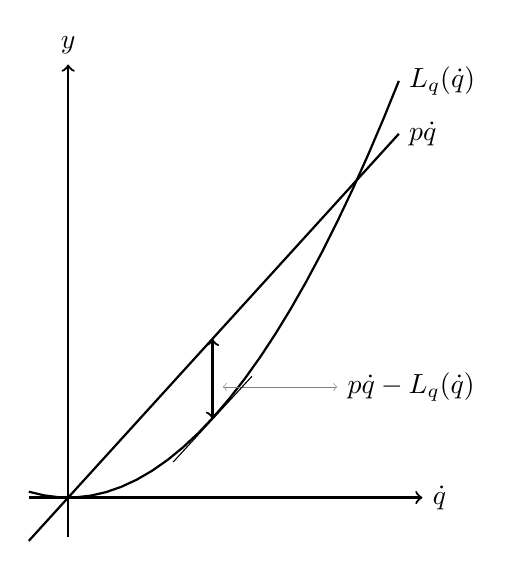
\begin{tikzpicture}
    \draw[->, thick] (-0.5, 0) -- (4.5, 0) node[anchor=west] {$\dot{q}$};
    \draw[->, thick] (0, -0.5) -- (0, 5.5) node[anchor=south] {$y$};
    
    \draw[thick, domain=-0.5:4.2] plot ({\x}, {0.3*\x*\x}) node[anchor=west] {$L_q(\dot{q})$};
    \draw[thick, domain=-0.5:4.2] plot ({\x}, {1.1*\x}) node[anchor = west] {$p\dot{q}$};
    
    \draw[<->, thick] (1.8333, 1) -- (1.8333, 2.01663) node[pos=0.4, pin={[right, xshift=1cm]0:{$p \dot{q} - L_q(\dot{q})$}}] {};
    
    \draw (1.8333, 1) ++(-0.5, -0.549) -- ++(1, 1.089);
    
\end{tikzpicture}
    \caption{Geometric illustration of the Legendre transform of a function. The Legendre transform of the function $L = L(q, \dot{q})$ is a function of $p$ and $q$, defined as the difference $p\dot{q} - L_q$, where this difference must be maximal with respect to $\dot{q}$. If $L$ is a convex function in $\dot{q}$, this is achieved where the partial derivative $\pdv*{L}{\dot{q}}$ evaluated at $\dot{q}$ is equal to $p$, which is equivalent to being locally parallel to $p\dot{q}$. Because the Legendre transform is supposed to be a function of $p$, one can consider $p$ as `given'. $L_q$ denotes $L$ as a function of $\dot{q}$, for some given $q$.} 
    \label{fig:my_label}
\end{figure}

The economic interpretation of the Legendre transform may be better understood geometrically. The Legendre transform of a function $L = L(q, \dot{q})$ with respect to $\dot{q}$ is alternatively defined as
\begin{equation}
    \max_{\dot{q}}\qty{p\dot{q} - L(q, \dot{q})}.
\end{equation}
If $L$ is convex in $\dot{q}$, this is achieved at the point where the function $L$ is locally parallel to the function $p\dot{q}$, which is to say that
\begin{equation}
    \left.\pdv{L}{\dot{q}}\right |_{\dot{q}} = p.
\end{equation}
In the Lagrangian formalism, this is the very \emph{definition} of $p$: if $L$ is convex, the maximization is satisfied by default and is often disregarded.

For the economic interpretation, it is important to keep in mind the underlying maximization in the definition: it states that firms or consumers automatically operate at the optimal price point, given their cost (or utility) function.

\subsection{Hamilton's equations} 
Hamilton's equations are derived by applying the symplectic isomorphism to the gradient of the Hamiltonian function, which is defined by the relation
\begin{equation}
    \dd{H} = \intpr{X_H}{\omega},
\end{equation}
or in alternative notation \(X_H = \fromDual{\omega}(\dd{H})\). Here, $\omega$ is the symplectic 2-form on $\ctbundle{Q}$ (cf. \cref{sec:symplectic_ee}). The symplectic isomorphism (and Hamilton's equations) are covered in greater detail in \cref{chap:geometric_structures}.

Conventionally, the symplectic 2-form is equal to $\wedgep{\dd{q}^i}{\dd{p}_i}$, and Hamilton's equations are:
\begin{equation}
    \dot{q}^i = \pdv{H}{p_i}, \qquad \qquad \dot{p}_i = -\pdv{H}{q^i}.
    \label{eq:legendre_trans_alternative}
\end{equation}
It is easy to see that these equations of motion are equivalent to the Euler-Lagrange equations, given that \(p_i = \pdv{L}{\dot{q}^i}\). We will go a lot more into detail on the (geometric) nature of Hamilton's equations in \cref{chap:geometric_structures}; the discussion here is limited to their interpretation in economic engineering.

The first Hamilton equation is equivalent to \emph{Hotelling's lemma}, which states that the demand for a particular good is that the supply (i.e. \(\dot{q}^i\)) of a good \(i\) is equal to the derivative of the profit function with respect to the price \(p_i\). It is usually emphasized that this is only the case when the price is the \emph{optimal} price for profit, but this is built into the definition of \(p_i\). As given by \cref{eq:legendre_trans_alternative}, the price value \(p_i = \pdv*{L}{\dot{q}^i}\) is exactly the one for which the profit function
\begin{equation}
     p_i\,\dot{q}^i - L,
\end{equation}
is maximized, provided \(L\) is convex in \(\dot{q}^i\). 

The second Hamilton equation provides the change in momentum or \emph{force}. In economic engineering, these forces are analogous to \emph{economic wants}, i.e. what drives a price up or down. The equation can be interpreted as the \emph{law of scarcity}, i.e. economic wants arise as a consequence of the stock levels/amount of goods in the system, pushing the price of the goods up or down.

\subsection{The role of dissipation} 
Traditional Hamiltonian and Lagrangian mechanics deal with conservative systems only; those that conserve the value of the total Hamiltonian. In economics, these would be systems that would, without external sources, always maintain the same level of profit. These types of conservative economic systems are just as hypothetical as their mechanical counterpart since there are \emph{always} elements present that limit the `efficiency' of an economic system, such as the depreciation of goods, consumption of goods, and transaction costs. 

Given the prominent role that the Hamiltonian and Lagrangian formalism play in the field of economic engineering, it is therefore essential to find a suitable way to include dissipative effects in the Hamiltonian and Lagrangian formalism (or an extension thereof), while still maintaining their economic interpretation. This is the subject of \cref{chap:geometric_structures}, and although it is formulated in terms of classical mechanics, the analogies described in this chapter may be readily used to substitute the mechanical quantities for their economic engineering counterparts. To that end, \cref{tab:analogies} provides an overview of the most important analogies used in economic engineering.

\renewcommand{\arraystretch}{1.3}
\begin{table}[ht]
    \centering
    \caption{Overview of some important analogies between economic engineering and mechanics.}
    \label{tab:analogies}
    \begin{tabular}{clclc}
        \toprule
        \textbf{Symbol} & \textbf{Mechanical variable} & \textbf{Units} & \textbf{Economic variable} & \textbf{Units} \\ 
        \midrule
            \(q\) & Displacement & \([\si{\meter}]\) & Quantity of goods & \([\si{\quantity}]\) \\ 
            \(\dot{q}\) & Velocity & \([\si{\meter\per\second}]\) & Flow of goods & \([\si{\quantity\per \year}]\) \\ 
            \(p\) & Momentum & \([\si{\kilogram \meter \per \second}]\) & Quantity of goods & \([\si{\money \per \quantity}]\) \\ 
            \(F\) & Force & \([\si{\kilogram \meter \per \second \squared}]\) & Economic want & \([\si{\money \per \quantity \per \year}]\) \\ 
            \(m\) & Mass & \([\si{\kilogram}]\) & Price elasticity & \([\si{\money \year \per \quantity \squared}]\) \\ 
            \midrule
            \(H\) & Hamiltonian / total energy & \([\si{\joule}]\) & Profit & \([\si{\money \per \year}]\) \\ 
            \(L\) & Lagrangian & \([\si{\joule}]\) & Running cost / disutility & \([\si{\money \per \year}]\) \\ 
        \bottomrule
    \end{tabular}
\end{table}
\renewcommand{\arraystretch}{1}

%<symbol: p> <expl: Price> <tags: letter,econ>
%<symbol: q> <expl: Quantity; amount of goods> <tags: letter,econ>
%<symbol: \dot{q}> <expl: Quantity demanded; quantity supplied; flow of goods> <tags: letter,econ>

